%------------------------------------------------------------------------------

\begin{frame}
  \frametitle{Analytical derivatives: $\left[\frac{\partial \Fbold}{\partial \ubold}\right]$}
  \begin{itemize}
  \item Derivative of numerical flux far from the immersed boundaries
  \begin{equation*}
    \frac{\partial \Fbold_{ij}}{\partial \ubold_{k}} = 
    {\color{red}{\frac{\partial \Fbold_{ij}}{\partial \wbold_{ij}}}} \,
    {\color{green}{\frac{\partial \wbold_{ij}}{\partial \wbold_k}}}\,
    \frac{\partial \wbold_k}{\partial \ubold_k}
  \end{equation*}
\item Contribution to the Jacobian due to the immersed boundary treatment
    \begin{equation*}
    \frac{\partial \Fbold_{ij}}{\partial \ubold_k} = 
    {\color{red}{\frac{\partial \Fbold_{ij}}{\partial \wbold_{ij}^\star}}} \,
    {\color{blue}{\frac{\partial \wbold_{ij}^\star}{\partial \wbold_k}}} \,
    \frac{\partial \wbold_k}{\partial \ubold_k} +
    {\color{red}{\frac{\partial \Fbold_{ij}}{\partial \wbold_{ij}}}} \,
    {\color{green}{\frac{\partial \wbold_{ij}}{\partial \wbold_k}}} \,
    \frac{\partial \wbold_k}{\partial \ubold_k}
    \end{equation*}
  \begin{itemize}
  \item {\color{red}{Analytical Jacobian of the (Roe's) numerical flux}}
  \item {\color{blue}{Analytical derivative of the solution of the 1D half-Riemann problem}}
  \item {\color{green}{Analytical derivative of MUSCL reconstruction and limitation}}  
  \end{itemize}
 \end{itemize}
\end{frame}

%------------------------------------------------------------------------------

\begin{frame}
  \frametitle{Analytical derivatives: $\left\{\frac{\partial \Fbold}{\partial \mubold}\right\}$}
  \begin{itemize}
  \item Effect of the geometry deformation on the numerical residual \\[1.5mm]
  \item Different from zero only for nodes closed to the immersed boundaries
    \begin{equation*}
      \Fbold_{ij} = \Fbold_{ij}(\wbold_{ij}, \wbold^\star_{ij}(\mubold), \n_{ij})
      \quad\longrightarrow\quad
      \pder{\Fbold_{ij}}{\mubold} = 
      \pder{\Fbold_{ij}}{\wbold^\star_{ij}}{\color{blue}{\pder{\wbold^\star_{ij}}{\mubold}}}
    \end{equation*} \vspace{-2.5mm}
    \item $\dfrac{\partial \wbold^\star_{ij}}{\partial \mubold}$ 
      involves derivatives w.r.t shape deformation parameter of\vspace{-4mm}
      \begin{columns}[t]
        \column{0.03\textwidth}
        \column{0.53\textwidth}
        \vspace{5mm}
        \begin{itemize}
        \item Linear extra/inter-polation of fluid states\\[-2mm]
        \item Pierce points coordinates\\[-2mm]
        \item Normal vector on the immersed surface\\[-2mm]
        \end{itemize}
        \column{0.45\textwidth}
        \begin{figure}[!ht]
          \centering
          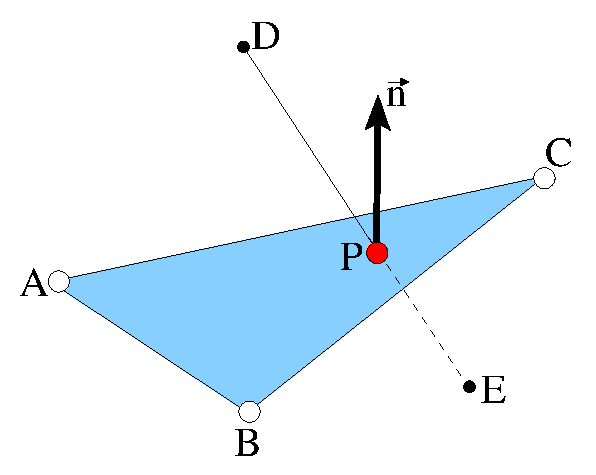
\includegraphics[width=0.65\linewidth]{Fig/pierce}
        \end{figure}
      \end{columns}\vspace{-4mm}
    \item Derivatives of geometrical quantities with respect to $\mubold$
      \begin{equation*}
        \frac{\partial \xi}{\partial \mubold} = 
        \frac{\partial \xi}{\partial x_\ell} \frac{\partial x_\ell}{\partial \mubold}, 
        \quad 
        \frac{\partial \boldsymbol{n}_{wall}}{\partial \mubold} = 
        \frac{\partial \boldsymbol{n}_{wall}}{\partial x_\ell} \frac{\partial x_\ell}{\partial \mubold},
        \quad \cdots
    \end{equation*}\vspace{-2.5mm}
    \item $\dfrac{\partial x_\ell}{\partial \mubold}$:
      Jacobian of the free-form deformation 
  \end{itemize}
\end{frame}

%------------------------------------------------------------------------------

\begin{frame}
  \frametitle{Analytical derivatives: $\left\{\frac{\partial \Jcal}{\partial s}\right\}$}
  \begin{itemize}
  \item Objective function: force coefficients  
    $\dfrac{\partial C_{L,D}}{\partial \mubold}$ and
    $\dfrac{\partial C_{L,D}}{\partial \ubold}$
    \item Aerodynamic forces computed by extrapolating pressure on the surface
      \begin{equation*}
        \boldsymbol{f} = \sum_{e \in E_r} P_e \boldsymbol{n}_e 
        \quad \Rightarrow \quad 
        C_L = \frac{\boldsymbol{f}\cdot \boldsymbol{\ell}}{q_\infty S}
        \quad,
        C_L = \frac{\boldsymbol{f}\cdot \boldsymbol{d}}{q_\infty S}
        \vspace{-1mm}
      \end{equation*}
      \item Derivative of the forces
        \begin{equation*}
          \begin{split}
            \frac{\partial \boldsymbol{f}}{\partial \mubold} & = 
            \sum_{e \in E_r} \frac{\partial P_e}{\partial P_i} \frac{\partial P_i}{\partial \mubold} \boldsymbol{n}_e  +
            \sum_{e \in E_r} P_e\frac{\partial  \boldsymbol{n}_e }{\partial \mubold} \\
            \frac{\partial \boldsymbol{f}}{\partial \ubold} & = 
            \sum_{e \in E_r} \frac{\partial P_e}{\partial P_i} \frac{\partial P_i}{\partial \ubold} \boldsymbol{n}_e 
          \end{split}
        \end{equation*}
\end{itemize}
\end{frame}